\documentclass[conf]{new-aiaa} % Use [journal] for AIAA journal style

%\usepackage[utf8]{inputenc}

%graphics packages
\usepackage[]{graphicx}
\graphicspath{{./figures/}}

% ------------------ tikz ------------
%%tikz
\RequirePackage{pgf,tikz, luatex85}
\usepackage{pgfplots}
\usepackage{booktabs} % in your preamble
\pgfplotsset{compat=newest}
\usetikzlibrary{arrows.meta}
\usetikzlibrary{arrows}
\usetikzlibrary{shapes.geometric}
\usetikzlibrary{shapes.misc}
\usetikzlibrary{backgrounds}
\usetikzlibrary{bending}
\usetikzlibrary{shadows}
\usetikzlibrary{patterns}
\usetikzlibrary{patterns.meta}
\usetikzlibrary{intersections}
\usepgfplotslibrary{patchplots}
\usepgfplotslibrary{fillbetween}
\usepgfplotslibrary{groupplots}
\usepgfplotslibrary{polar}
\usepgfplotslibrary{smithchart}
\usepgfplotslibrary{statistics}
\usepgfplotslibrary{dateplot}
\usepgfplotslibrary{ternary}


\pgfplotsset{%
	layers/standard/.define layer set={%
		background,axis background,axis grid,axis ticks,axis lines,axis tick labels,pre main,main,axis descriptions,axis foreground%
	}{grid style= {/pgfplots/on layer=axis grid},%
		tick style= {/pgfplots/on layer=axis ticks},%
		axis line style= {/pgfplots/on layer=axis lines},%
		label style= {/pgfplots/on layer=axis descriptions},%
		legend style= {/pgfplots/on layer=axis descriptions},%
		title style= {/pgfplots/on layer=axis descriptions},%
		colorbar style= {/pgfplots/on layer=axis descriptions},%
		ticklabel style= {/pgfplots/on layer=axis tick labels},%
		axis background@ style={/pgfplots/on layer=axis background},%
		3d box foreground style={/pgfplots/on layer=axis foreground},%
	},
}
% new style at automates partial ellipse
\tikzset{
    partial ellipse/.style args={#1:#2:#3}{
        insert path={+ (#1:#3) arc (#1:#2:#3)}
    }
}

\usepackage{caption}
\usepackage{subcaption}
\usepackage{placeins}
\usepackage{wrapfig}
\usepackage{url}
\usepackage{hyperref}

%tables
\usepackage{array}
\newcommand{\PreserveBackslash}[1]{\let\temp=\\#1\let\\=\temp}
\newcolumntype{C}[1]{>{\PreserveBackslash\centering}m{#1}}
\newcolumntype{R}[1]{>{\PreserveBackslash\raggedleft}m{#1}}
\newcolumntype{L}[1]{>{\PreserveBackslash\raggedright}m{#1}}

%mathpackages
\usepackage{amsmath}
%\usepackage{siunitx}
%\usepackage{mathrsfs}
%\newcommand{\vect}{\overset{\rightharpoonup}}
%decrease overset height
% \makeatletter
% \newcommand{\oset}[3][0.25ex]{%
% 	\mathrel{\mathop{#3}\limits^{
% 			\vbox to#1{\kern-0.5\ex@
% 				\hbox{$\scriptstyle#2$}\vss}}}}
% \makeatother

%%Vector arrow over variable
%\newcommand{\vect}[1]{%
%	\oset{\rightharpoonup}{#1}}

\RequirePackage{bm}
\newcommand{\vect}[1]{\bm{#1}}

\newcommand{\mat}[1]{%
	\mathbf{#1}}
\usepackage{nicefrac}
\usepackage{cancel}

%referencing packages
\usepackage[]{cleveref}
\usepackage{hyperref}
\usepackage{float}
\usepackage{placeins}

% ---------- colors -------------
\RequirePackage{xcolor}
\definecolor{navy}{HTML}{002E5D}
\definecolor{royal}{HTML}{005CAB}	% royal that matches BYU Engineering logo
\definecolor{darkgray}{HTML}{141414}
\definecolor{mediumgray}{HTML}{666666}	% medium gray definition from A. Ning
\definecolor{black}{HTML}{111111}
\definecolor{primary}{HTML}{005CAB}
\definecolor{secondary}{HTML}{c05367}
\definecolor{tertiary}{HTML}{8fa651}
\definecolor{plotsgray}{HTML}{808080}


% -------------- easy coloring of things ----------------
\newcommand{\navy}[1]{{\color{navy}#1}}
\newcommand{\primary}[1]{{\color{primary}#1}}
\newcommand{\secondary}[1]{{\color{secondary}#1}}
\newcommand{\tertiary}[1]{{\color{tertiary}#1}}
\newcommand{\gray}[1]{{\color{gray}#1}}

% Allow same footnotes
\newcommand*\samethanks[1][\value{footnote}]{\footnotemark[#1]}

% make \noindent where easier
\newcommand{\where}{\noindent where }
 % your preamble.tex file with packages

\begin{document}
\sloppy % helps reduce overfull hboxes

\title{Lab 1: A Tensile Test on 1018 Steel and 6061 Aluminum}
\author{Nathan R. Lehnhof\footnote{Mechanical Engineering}}
\affil{BYU Provo, UT}
\date{\today}
\maketitle

% ======================================================
\begin{abstract}
Lab 1 determines the value of the ultimate strength, yield strength, and the modulus of elasticity of Steel 1018 (cold rolled) and 6061 Aluminum by performing tensile tests.
Ultimate strength is the maximum stress a material can withstand before noticable necking.
It's the maximum point on the engineering stress-strain curve.
Yield stress is the stress at which the material begins to noticibly plastically deform, defined at 0.002 strain.
Young's Modulus of Elasticity is the measure of a material's stiffness, being the slope of the elastic region of the stress-strain graph.
\end{abstract}

% ======================================================
\section{Methods}
To perform the tensile test, Steel 1018 and 6061 Aluminum "dog-bones" were placed in the tensile tester.
The "dog-bones" had a diameter of 0.3 inches (7.62 mm) and a gauge length of 2.3 inches (58.42 mm).
The tensile tester than gradually increased the tensile force experienced by the specimens, recording the force and the length of the specimen.
The data was returned as an excel file.
Because the tensile tester takes data so quickly, the last few data points of the file are after fracture, so those are manually removed.
Similarly, the tensile tester secures the samples with clamps.
That clamping produces an initial compressive force that is also measured.
Those points are also manually removed in data post-processing.

\begin{align}
    \sigma &= \frac{F}{A} \label{stress}
    && \text{Stress (MPa)} \\[6pt]
    \epsilon &= \frac{\delta l}{l_0} \label{strain} 
    && \text{Strain}
\end{align}

Since we need stress and strain, we use \autoref{stress} and \autoref{strain}.
From the Force (N) and diameter (mm), we find stress by dividing the force by the initial cross-sectional area.
To find strain, we first need to normalize our length, taking the first length as 0.0.
Then, we can use \autoref{strain} to find strain.
We then graph stress-strain for both Steel 1018 and 6061 Aluminum.
From the results, we can determine young's modulus (GPa), yield stress (MPa), and ultimate tensile stress (MPa) as shown in the following figures and tables.

% ======================================================
\section{Results}

\begin{figure}[H]
    \centering
    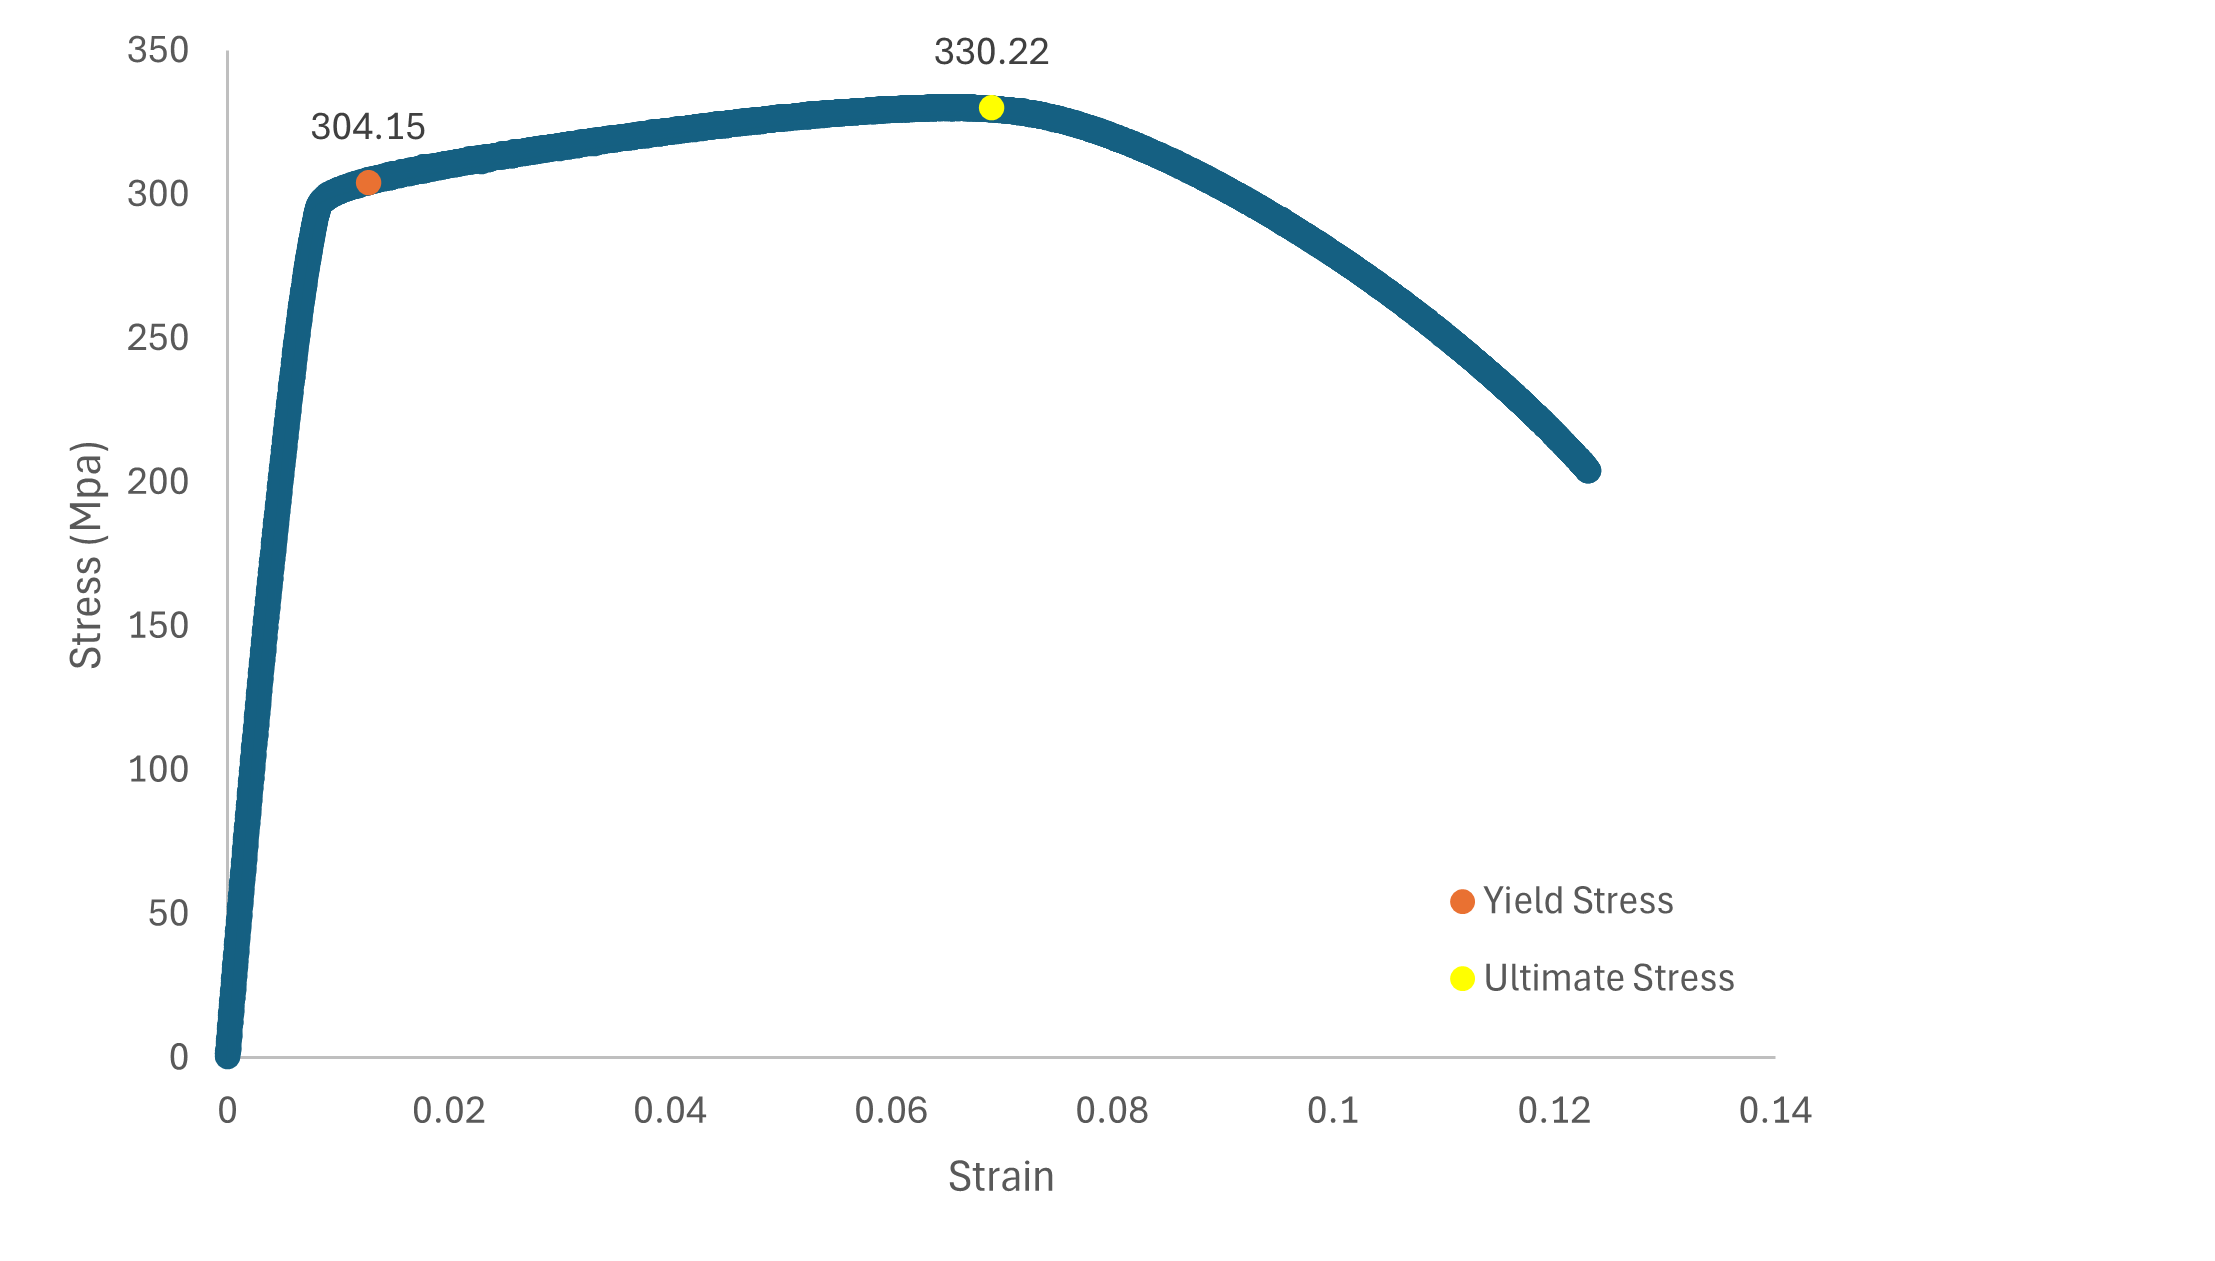
\includegraphics[width=0.7\linewidth]{alxl.png}
    \caption{Stress-strain curve for 6061 Aluminum.}
    \label{fig:aluminum}
\end{figure}

\begin{table}[H]
    \centering
    \renewcommand{\arraystretch}{1.3}
    \begin{tabular}{lcc}
    \toprule
    \textbf{6061 Aluminum} & Expected & Actual \\
    \midrule
    Ultimate Strength (MPa) & 330 & 310 \\ 
    Yield Strength (MPa)    & 304 & 276 \\ 
    Modulus $E$ (GPa)       & 69  & 69 \\ 
    \bottomrule
    \end{tabular}
    \caption{Mechanical properties of 6061 Aluminum.}
    \footnotesize\textit{Data for expected values from \cite{matweb6061}.}
    \label{tab:aluminum}
\end{table}

\begin{figure}[H]
    \centering
    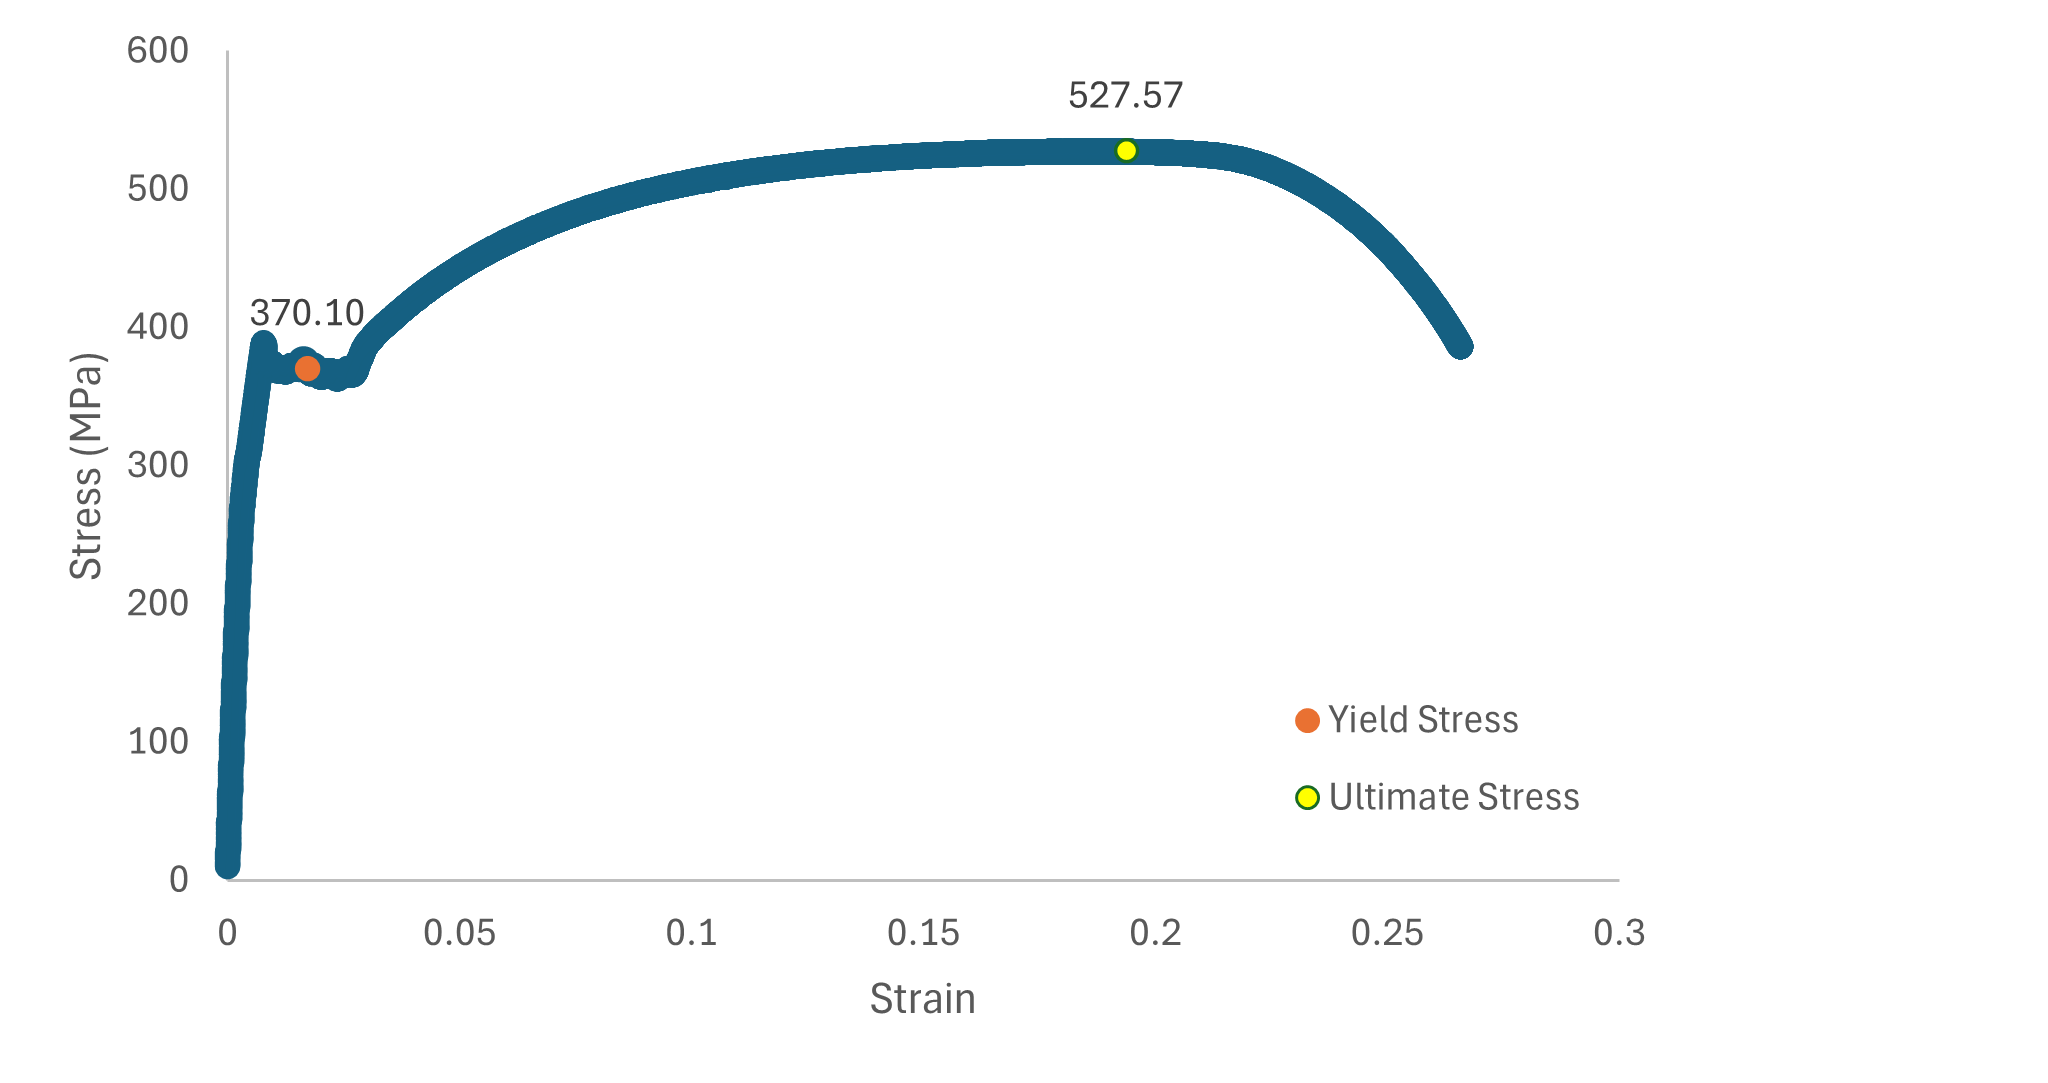
\includegraphics[width=0.7\linewidth]{stxl.png}
    \caption{Stress-strain curve for Steel 1018 Cold-Rolled.}
    \label{fig:steel}
\end{figure}

\begin{table}[H]
    \centering
    \renewcommand{\arraystretch}{1.3}
    \begin{tabular}{lcc}
    \toprule
    \textbf{Steel 1018} & Expected & Actual \\
    \midrule
    Ultimate Strength (MPa) & 528 & 440 \\ 
    Yield Strength (MPa)    & 370 & 370 \\ 
    Modulus $E$ (GPa)       & 217 & 205 \\ 
    \bottomrule
    \end{tabular}
    \caption{Mechanical properties of Steel 1018.}
    \footnotesize\textit{Data for expected values from \cite{matweb1018}.}
    \label{tab:steel}
\end{table}

\noindent\footnotesize\textit{Note: Young’s Modulus for both materials was calculated numerically by averaging the slope of the stress–strain curve in the initial linear-elastic region.}

\FloatBarrier

% ======================================================
\section{Conclusion}
We are more interested in the stress-strain curve than a force-displacement curve because stress and strain allows us to calculate yield stress, ultimate tensile stress, and Young's elastic modulus.
A force and displacement graph only works for the specific geometry of the dog-bone.
The stress-strain graph reflects the material properties that can be used with a range of geometries.
The values calculated from the stress-strain graph can be used universally with that material.

True stress uses the instantaneous area; true strain uses the instantaneous change in length.
While true stress/strain reflect more accurate properties, true stress/strain tests are more costly.
Engineering stress and strain is sufficient for engineering purposes.
A tensile test would be necessary for the following: space vehicle separation bolts, suspension bridge cables or truss members, lifting equiment, fasteners under tension, cables for elevators/cranes.
An engineer designing the cables on a suspension bridge would want to know the tensile properties of the cable material to ensure it can handle the expected loads.
Similarly, an engineer designing a ship's anchor would want to know the tensile properties of the anchor chain.

The measured ultimate strength of 6061 Aluminum (310 MPa) was close to the
published value of 330 MPa from MatWeb \cite{matweb6061}, while the measured
ultimate strength of 1018 steel (440 MPa) was lower than the expected 528 MPa
\cite{matweb1018}. From the data we can see that Steel 1018 is significantly stronger (Ultimate Stress) and stiffer (Young's Modulus) than Aluminum 6061, which is expected.
Aluminum 6061 and Steel 1018 have similar yield strengths, with Aluminum being slightly lower.

Some potential sources of error include machine calibration (unlikely), misalignment of dog-bones (more likely since it would change the gauge length), and the machining of the dog-bones (could introduce heat/properties into the material).
Another important point is that this is only one sample.
As the number of samples increases, the accuracy of our values will increase.
We can most likely reduce error by increasing the number of tests and increasing consistency in machining the dog-bones.

\section{References and Resources}

% \nocite{*}
\bibliographystyle{new-aiaa}
\bibliography{references}

\end{document}
